
\subsection{Listoj}

%%%>>>>>>>>>>>>>>>>>>>>>>>>>>>>>>>>>>>>>>>>>>>>>>>>>>>>>>>>>>>>>>>>>>>>>>>>>>>>>>>>>>>>>>>>>>>>>>
  \begin{frame}
    \frametitle{Kio sekve?}
    \framesubtitle{Listoj}

	La tabulo estas nur rimedo, kio ech pli gravas estas metodaro: tiel nomata  \textbf{laborfluo}. Ghi difinas kiajn listojn ni havas sur la tablo kaj kiel transmeti la kartojn inter ili.
	
  \end{frame}
%%%<<<<<<<<<<<<<<<<<<<<<<<<<<<<<<<<<<<<<<<<<<<<<<<<<<<<<<<<<<<<<<<<<<<<<<<<<<<<<<<<<<<<<<<<<<<<<<

%%%>>>>>>>>>>>>>>>>>>>>>>>>>>>>>>>>>>>>>>>>>>>>>>>>>>>>>>>>>>>>>>>>>>>>>>>>>>>>>>>>>>>>>>>>>>>>>>
  \begin{frame}
    \frametitle{Listoj: ekzemploj de laborfluoj}
    \framesubtitle{La unua provo}
    
    	\begin{columns}
    \column{0.3\textwidth}
	    \begin{block}
	    
	    	Far\alert{ot}aj
	    	
	    \end{block}
	\column{0.3\textwidth}
    	\begin{block}
    	
    		Far\alert{at}aj
    		
   		\end{block}
	\column{0.3\textwidth}
    	\begin{block}
    	
    		Far\alert{it}aj
    		
    	\end{block}
	\end{columns}
    \vspace{1em}
    	\begin{columns}
    \column{0.5\textwidth}
    Avantaghoj:
    \begin{itemize}
    		\item simpla
    \end{itemize}
	\column{0.5\textwidth}
    Difektoj:
    \begin{itemize}
    		\item malklara diferenco inter Farotaj kaj Farataj,
    		\item Mankas loko por novaj ideoj, ne nepre tuj farindajn -  ideoj ,,poluas'' nunajn urghajn taskojn.
    \end{itemize}
    	
	\end{columns}
  \end{frame}
%%%<<<<<<<<<<<<<<<<<<<<<<<<<<<<<<<<<<<<<<<<<<<<<<<<<<<<<<<<<<<<<<<<<<<<<<<<<<<<<<<<<<<<<<<<<<<<<<


%%%>>>>>>>>>>>>>>>>>>>>>>>>>>>>>>>>>>>>>>>>>>>>>>>>>>>>>>>>>>>>>>>>>>>>>>>>>>>>>>>>>>>>>>>>>>>>>>
  \begin{frame}
    \frametitle{Listoj: ekzemploj de laborfluoj}
    \framesubtitle{Dua provo}
    
    	\begin{columns}
    \column{0.3\textwidth}
	    \begin{block}
	    
	    	Ideoj
	    
    	\end{block}
	\column{0.3\textwidth}
    	\begin{block}
    	
    		Aktualaj
    	
    	\end{block}
	\column{0.3\textwidth}
    	\begin{block}
    	
    		Faritaj
    		
    	\end{block}
    	
	\end{columns}
    \vspace{4em}
    	\begin{columns}
    \column{0.5\textwidth}
    Avantaghoj:
    \begin{itemize}
    		\item Ideoj: loko por cerbshtormetoj
    		\item Aktualaj: la situacio klaras
    \end{itemize}
	\column{0.5\textwidth}
    Difektoj:
    \begin{itemize}
    		\item Aktualaj povas kreski tro longa!
    \end{itemize}
    	
	\end{columns}
  \end{frame}
%%%<<<<<<<<<<<<<<<<<<<<<<<<<<<<<<<<<<<<<<<<<<<<<<<<<<<<<<<<<<<<<<<<<<<<<<<<<<<<<<<<<<<<<<<<<<<<<<




%%%>>>>>>>>>>>>>>>>>>>>>>>>>>>>>>>>>>>>>>>>>>>>>>>>>>>>>>>>>>>>>>>>>>>>>>>>>>>>>>>>>>>>>>>>>>>>>>
  \begin{frame}
    \frametitle{La plej bona solvo?}
    
    		\begin{center}
    		\begin{block}
    		
			\begin{huge}
				\begin{center}
				Estu \alert{fleksebla}!
				\end{center}
			\end{huge} 
    		\end{block}

			\vspace{1.5em}    		
    		
    		
\includegraphics[scale=0.5]{meme/kato}
    		
    		\end{center}

  \end{frame}
%%%<<<<<<<<<<<<<<<<<<<<<<<<<<<<<<<<<<<<<<<<<<<<<<<<<<<<<<<<<<<<<<<<<<<<<<<<<<<<<<<<<<<<<<<<<<<<<<


%%%>>>>>>>>>>>>>>>>>>>>>>>>>>>>>>>>>>>>>>>>>>>>>>>>>>>>>>>>>>>>>>>>>>>>>>>>>>>>>>>>>>>>>>>>>>>>>>
  \begin{frame}
    \frametitle{La plej bona solvo?}
    
    		\begin{center}
    		\begin{block}
    		
			\begin{huge}
				\begin{center}
				\alert{Eksperimentu}!
				\end{center}
			\end{huge} 
    		\end{block}

			\vspace{1em}    		
    		
    		
\includegraphics[scale=0.35]{meme/eksperimento}
    		
    		\end{center}

  \end{frame}
%%%<<<<<<<<<<<<<<<<<<<<<<<<<<<<<<<<<<<<<<<<<<<<<<<<<<<<<<<<<<<<<<<<<<<<<<<<<<<<<<<<<<<<<<<<<<<<<<


%%%>>>>>>>>>>>>>>>>>>>>>>>>>>>>>>>>>>>>>>>>>>>>>>>>>>>>>>>>>>>>>>>>>>>>>>>>>>>>>>>>>>>>>>>>>>>>>>
  \begin{frame}
    \frametitle{Fleksebla?}
    \framesubtitle{Datumoj listo}
    
    
    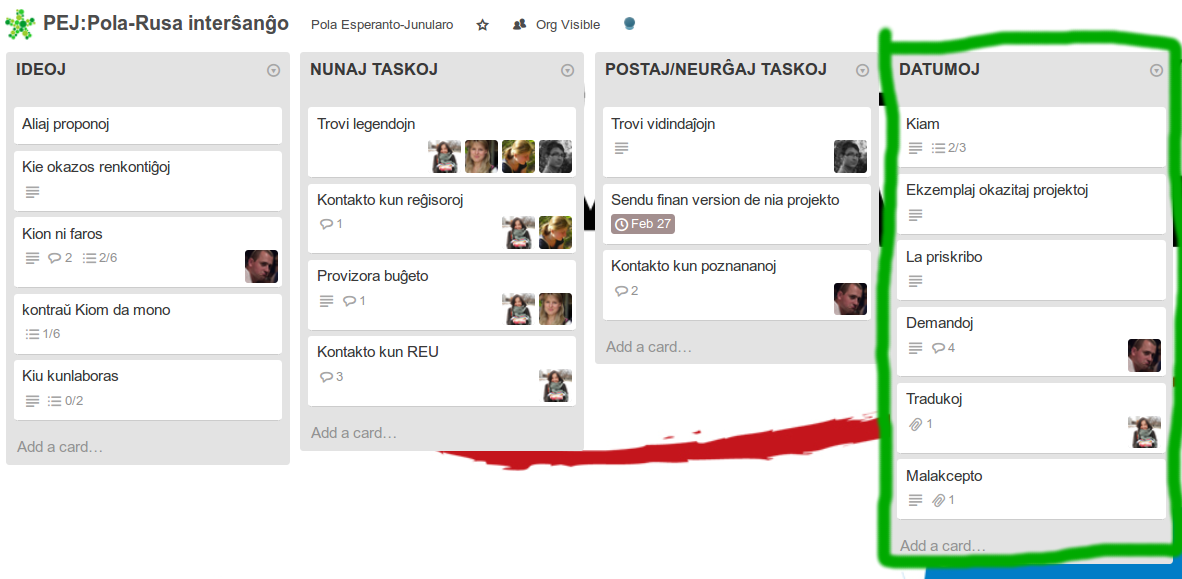
\includegraphics[scale=0.25]{ekranoj/datumoj}

  \end{frame}
%%%<<<<<<<<<<<<<<<<<<<<<<<<<<<<<<<<<<<<<<<<<<<<<<<<<<<<<<<<<<<<<<<<<<<<<<<<<<<<<<<<<<<<<<<<<<<<<<


%%%>>>>>>>>>>>>>>>>>>>>>>>>>>>>>>>>>>>>>>>>>>>>>>>>>>>>>>>>>>>>>>>>>>>>>>>>>>>>>>>>>>>>>>>>>>>>>>
  \begin{frame}
    \frametitle{Fleksebla?}
    \framesubtitle{Listo por priparolindaj aferoj dum skajpa kunsido}
    
    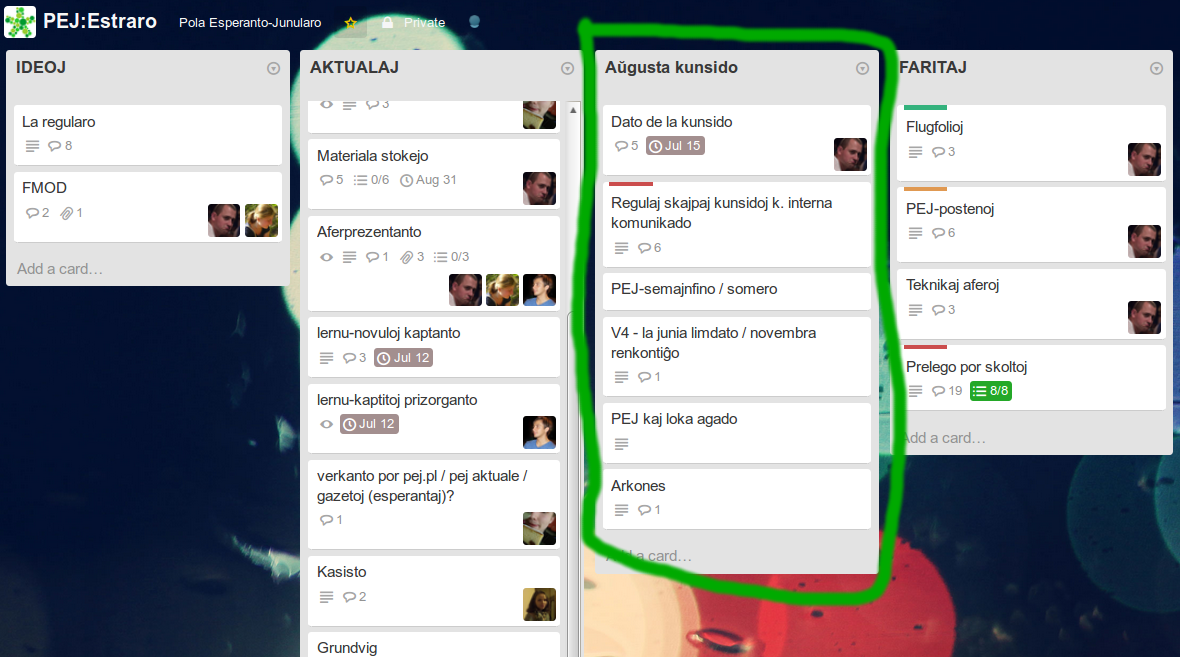
\includegraphics[scale=0.25]{ekranoj/augusta-kunsido}

  \end{frame}
%%%<<<<<<<<<<<<<<<<<<<<<<<<<<<<<<<<<<<<<<<<<<<<<<<<<<<<<<<<<<<<<<<<<<<<<<<<<<<<<<<<<<<<<<<<<<<<<<


%%%>>>>>>>>>>>>>>>>>>>>>>>>>>>>>>>>>>>>>>>>>>>>>>>>>>>>>>>>>>>>>>>>>>>>>>>>>>>>>>>>>>>>>>>>>>>>>>
  \begin{frame}
    \frametitle{Fleksebla?}
    \framesubtitle{Listoj kun programoj por ĉiu tago de aranĝo}
    
    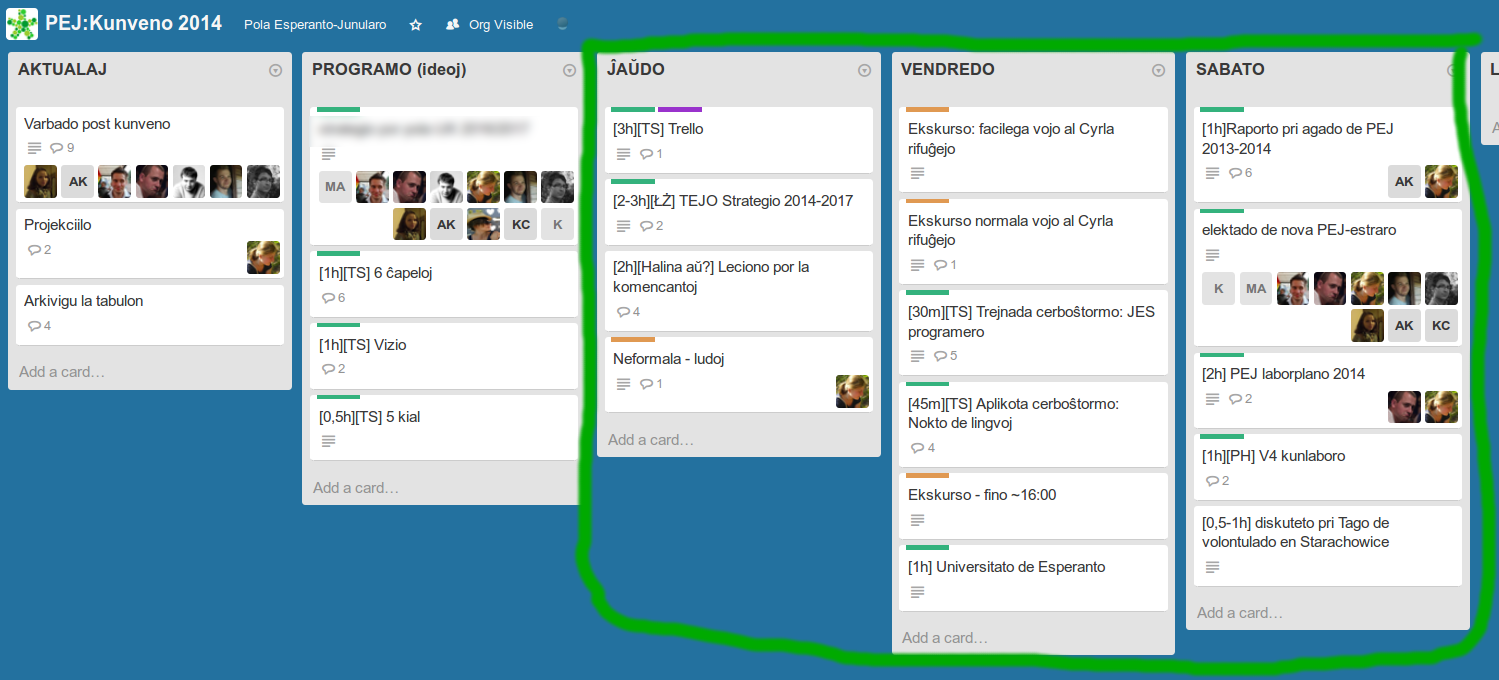
\includegraphics[scale=0.21]{ekranoj/programo-listoj}
  \end{frame}
%%%<<<<<<<<<<<<<<<<<<<<<<<<<<<<<<<<<<<<<<<<<<<<<<<<<<<<<<<<<<<<<<<<<<<<<<<<<<<<<<<<<<<<<<<<<<<<<<
